% 为了满足 2026 年上传要求可以选择不生成封面和编号页，参考这里
% 参考这里：https://cumcm.cnki.net/cumcm/studentHome/noticeDetail?id=c0c5220f-0226-4cd8-bce1-e1f81e1e23f6

%\documentclass{cumcmthesis}

\documentclass[withoutpreface,bwprint]{cumcmthesis} %去掉封面与编号页，电子版提交的时候使用。

\usepackage[most]{tcolorbox}
\usepackage{tikz}
\usepackage{cumcm2026}

\newtcolorbox{framee}[1][]{
  enhanced,
  skin=enhancedlast jigsaw,
  attach boxed title to top left={xshift=-4mm,yshift=-0.5mm},
  fonttitle=\bfseries\sffamily,
  colbacktitle=blue!45,
  colframe=red!50!black,
  interior style={
    top color=blue!10,
    bottom color=red!10
  },
  boxed title style={
    empty,
    arc=0pt,
    outer arc=0pt,
    boxrule=0pt
  },
  underlay boxed title={
    \fill[blue!45!white]
      (title.north west) --
      (title.north east) --
      +(\tcboxedtitleheight-1mm,-\tcboxedtitleheight+1mm) --
      ([xshift=4mm,yshift=0.5mm]frame.north east) --
      +(0mm,-1mm) --
      (title.south west) -- cycle;
    \fill[blue!45!white!50!black]
      ([yshift=-0.5mm]frame.north west) --
      +(-0.4,0) --
      +(0,-0.3) -- cycle;
    \fill[blue!45!white!50!black]
      ([yshift=-0.5mm]frame.north east) --
      +(0,-0.3) --
      +(0.4,0) -- cycle;
  },
  title={2026 年建模比赛格式变化说明},
  #1
}

\usepackage{url}   % 网页链接
\usepackage{subcaption} % 子标题
\title{全国大学生数学建模竞赛编写的 \LaTeX{} 模板}

%%=======如下信息已经不再需要填写========
\tihao{A}
\baominghao{4321}
\schoolname{XX大学}
\membera{ }
\memberb{ }
\memberc{ }
\supervisor{ }%辅导老师
\yearinput{2026}
\monthinput{9}
\dayinput{1}
%===================================

\begin{document}

% ===== BEGIN B26 NEW MANUSCRIPT: safe to edit this block =====
\begingroup
\setlength{\emergencystretch}{2em}
% Preserve the template's printed spacing while giving PDF bookmarks plain numbers.
\renewcommand{\thesubsection}{\texorpdfstring{\arabic{section}\thinspace.\thinspace\arabic{subsection}}{\arabic{section}.\arabic{subsection}}}
\renewcommand{\thesubsubsection}{\texorpdfstring{\thesubsection\thinspace.\thinspace\arabic{subsubsection}}{\arabic{section}.\arabic{subsection}.\arabic{subsubsection}}}
\begin{center}
{\heiti\zihao{3}\bfseries 无线电干扰源的有界误差定位与主动测向选点\par}
\vspace{0.6em}
{\small 论文正文阶段稿：问题分析与第一、二问\par}
\end{center}
\vspace{0.5em}
% B26 manuscript body: problem analysis and solutions to Problems 1 and 2.
% Required packages: amsmath, amssymb, booktabs, tikz.
% All numerical examples in this file are synthetic, not official test results.

\section{问题重述}
\subsection{研究背景}
无线电干扰源的精准定位与清除是无线电频谱管理的重要环节。大范围监测虽然能够确定目标的大致分布区域，但在环境遮挡、干扰源功率不同以及测向误差的共同影响下，仍需移动设备进入目标区域进行交会测向和近距离确认。采用搭载测向机、光学探测仪和激光清除装置的机器狗，可以将人工逐点排查转化为自动搜索与决策问题。

题目给定干扰源位于半径为 $1800\,\mathrm{m}$ 的圆域内，以圆心为原点，正东、正北分别为 $x$、$y$ 轴正方向。不同干扰源占用互不相同的频道，频道编号为 $1$ 至 $20$。每个源的有效接收半径介于 $1000\,\mathrm{m}$ 与 $1500\,\mathrm{m}$ 之间，具体数值未知。正常测向读数相对真实方位角的误差不超过 $1^\circ$；同一地点重复测量不会改变误差。

机器狗以 $5\,\mathrm{m/s}$ 的速度沿直线移动，停车检测一次耗时 $5\,\mathrm{s}$，切换频道耗时 $1\,\mathrm{s}$。在距目标不超过 $20\,\mathrm{m}$ 的位置，可进行耗时 $3\,\mathrm{s}$ 的光学精确定位并用 $2\,\mathrm{s}$ 清除目标。若接收到信号且距离不超过 $5\,\mathrm{m}$，测向机返回近场反馈，可直接进入清除阶段。这些条件表明，定位精度与运动代价必须共同纳入算法设计。

\subsection{待解决的问题}
\begin{enumerate}
  \item 根据同一干扰源在若干检测点的示向度，建立有界误差下的多边形定位区域，给出其直径计算算法，并判断是否存在同直径圆覆盖该区域。
  \item 在仅有一次全向源正常测向读数的条件下，确定第二检测点的候选区域，提出兼顾接收可靠性、交会精度和移动代价的选点策略。
  \item 对总数未知但位于 $10$ 至 $16$ 个之间的全向源，设计从原点出发的自动搜索、定位和清除策略，在完整清除的约束下减少总用时。
  \item 将上述任务推广到全向源与定向源混合的情形，处理源类型和发射朝向未知所带来的检测盲区。
\end{enumerate}
前两问研究局部交会几何与主动选点，为后两问的搜索、定位及清除调度提供基础。下文首先完成问题分析及前两问的模型建立与求解。

\section{问题分析}
\subsection{问题一：由角度误差到集合定位}
一次示向度并不对应唯一射线，而对应张角为 $2^\circ$ 的向前角域。多次有效观测所允许的位置为这些角域的交集。由于每个角域均可写成两个闭半平面，其交集是凸集，可以用半平面求交及凸包算法求解。首先需要判断交集是否为空或无界，再讨论有限直径，否则人为设置的计算边框可能将无界区域误判成有限定位结果。

区域直径描述两个可能位置之间的最大距离；光学清除则要求存在一个机器人停靠点，使所有可能位置到它的距离均不超过 $20\,\mathrm{m}$。二者对应不同的几何量。因此，问题一不仅要计算最远点对，还要分析最小包围圆与区域直径的关系，建立可供后续清除决策使用的判据。

\subsection{问题二：保证接收与交会几何的共同约束}
第二检测点若离首站过近，或近似位于首次示向线上，两条视线可能几乎平行，难以消除沿首方向的距离不确定性；若横向偏移过大，则可能超出目标的有效接收范围。有效半径未知，使得单纯追求较大的交会角并不足以构成可靠策略。

首次成功接收还蕴含了半径信息：若真实目标距首站为 $r$，其接收半径至少为 $\max(1000,r)$。据此可先构造对所有可能目标均保证接收的第二站集合，再在该集合内比较候选点的后验不确定半径和移动距离。题目未给出误差的概率分布，因此采用集合意义下的稳健评价，不将等权采样均值解释成真实环境下的期望误差。

\subsection{全任务的时间目标及前两问的作用}
设总移动距离为 $L_{\mathrm{tot}}$，检测、切换频道、光学尝试和成功清除的次数分别为 $N_{\mathrm{m}}$、$N_{\mathrm{s}}$、$N_{\mathrm{o}}$、$N_{\mathrm{c}}$，题目虚拟总时间可写为
\begin{equation}
 T=\frac{L_{\mathrm{tot}}}{5}+5N_{\mathrm{m}}+N_{\mathrm{s}}+3N_{\mathrm{o}}+2N_{\mathrm{c}}.
 \label{eq:b26-time}
\end{equation}
其中失败的光学尝试也计入 $N_{\mathrm{o}}$；清除指令不改变测向机当前频道，不能额外计为一次频道切换。程序实际运行时间与上述虚拟时间分别统计。

由式~\eqref{eq:b26-time}可知，增加一次测向是否值得，需要比较其减少的后续移动和光学搜索时间。问题一给出可靠的停止定位判据，问题二提供有效的下一站选择方法；两者共同服务于全任务用时目标。对于定向源，无信号还可能来自发射方向遮挡，不能直接解释成目标不在附近，因此问题二的全向接收保证不能原样推广到问题四。

\section{模型假设与约定}
\begin{enumerate}
 \item 按题目二维模型处理源与机器狗的位置，在一次定位过程中目标位置、频道、有效接收半径及发射特征保持不变。
 \item 正常测向误差仅满足确定性界 $|\varepsilon_i|\leq1^\circ$；不假设其服从正态分布，也不假设同地点重复测量产生独立样本。
 \item 问题一的定位区域仅指闭角域交集。目标圆域和接收距离可在后续选点中作为附加先验，但不用于悄悄截断问题一的无界集合。
 \item 问题二限定目标为尚未清除的全向源。无信号、近场及正常示向度分别处理，缺失的示向度不作为角度零值输入模型。
 \item 理论推导使用 $\alpha=1^\circ$。接口保留两位小数，数值示例按舍入最大增加 $0.005^\circ$ 的保守方式取 $\bar\alpha=1.005^\circ$；这是一项实现余量，并非修改题面误差。
 \item 数值算例为明确设置的合成数据，仅用于验证公式与比较候选策略；不代表正式测试成绩，也不作为连续最优性的证明。
\end{enumerate}

\section{符号说明}
\begin{table}[H]
 \centering
 \caption{主要符号及含义}\label{tab:b26-symbols}
 \begin{tabular}{cl}
 \toprule
 符号 & 含义 \\
 \midrule
 $g,\ s_i,\ q$ & 真实目标位置、第 $i$ 个检测点、待选第二检测点 \\
 $\theta_i,\alpha$ & 示向度及理论角误差上界 \\
 $R$ & 目标的未知有效接收半径，$1000\leq R\leq1500$ \\
 $W_i,\ P$ & 第 $i$ 个观测角域及其交集 \\
 $K,\widehat K$ & 加入距离先验的可行域及其保守多边形外近似 \\
 $D$ & 定位区域的直径 \\
 $c^*,R^*$ & 最小包围圆的圆心与半径 \\
 $u,v$ & 首次示向的单位向量及其左法向量 \\
 $\mathcal G$ & 首次正常反馈后的可能目标集合 \\
 $\mathcal C_{\mathrm{recv}},\mathcal C_4$ & 保证接收集合及四圆候选集合 \\
 $a,b,L$ & 第二站纵向、横向位移及设计移动预算 \\
 $J(q),\widehat J(q)$ & 连续最坏后验半径及其采样评分 \\
 \bottomrule
 \end{tabular}
\end{table}
除特别说明外，距离单位为米、时间单位为秒。记 $\overline B(c,r)=\{x:\|x-c\|_2\leq r\}$；二维叉积定义为 $a\times b=a_xb_y-a_yb_x$。涉及角度线性化时，角误差使用弧度制。

\section{问题一：交会定位区域的直径与覆盖圆}
\subsection{观测角域的半平面表示}
对于位置 $s_i=(x_i,y_i)^{\mathsf T}$ 处的正常示向度 $\theta_i$，定义边界方向
\begin{equation}
 u_i^- =\begin{pmatrix}\cos(\theta_i-\alpha)\\ \sin(\theta_i-\alpha)\end{pmatrix},\qquad
 u_i^+ =\begin{pmatrix}\cos(\theta_i+\alpha)\\ \sin(\theta_i+\alpha)\end{pmatrix}.
\end{equation}
其闭角域为
\begin{equation}
 W_i=\{x:u_i^-\times(x-s_i)\geq0,\quad u_i^+\times(x-s_i)\leq0\}.
 \label{eq:b26-wedge}
\end{equation}
两条有向约束同时成立，才能保留向前张开的角域并排除反向区域。三角函数表示还能自然处理 $0^\circ$ 与 $360^\circ$ 附近的跨界读数。

将式~\eqref{eq:b26-wedge}写成矩阵形式，有
\begin{equation}
 A_i=\begin{pmatrix}
 \sin(\theta_i-\alpha)&-\cos(\theta_i-\alpha)\\
 -\sin(\theta_i+\alpha)&\cos(\theta_i+\alpha)
 \end{pmatrix},\qquad b_i=A_i s_i.
\end{equation}
叠加 $n$ 次观测，得到由 $2n$ 个半平面描述的定位区域
\begin{equation}
 P=\bigcap_{i=1}^nW_i=\{x:Ax\leq b\}.
 \label{eq:b26-region}
\end{equation}
该定义按交会几何取闭包，不额外挖去检测点周围的 $5\,\mathrm{m}$ 圆盘。若加入近场排除信息，集合可能不再是凸多边形，需另行处理。

\subsection{区域分类与顶点求解算法}
首先归一化各约束的法向量，并求解线性可行性问题 $Ax\leq b$。若不可行，则输出空集及观测不一致提示，不以直径零代替。若可行，分别求解 $x$、$-x$、$y$、$-y$ 四个方向的线性最小化问题；任一目标无界时，$P$ 无界，其直径为 $+\infty$。四个坐标方向均有界，则 $P$ 是有界闭凸集。

对于非空有界情形，采用如下可审计的基准算法。
\begin{enumerate}
 \item 枚举两条不平行的边界直线，求解对应的 $2\times2$ 线性方程组。
 \item 检查交点是否满足全部 $2n$ 个约束，只保留可行交点；按明确的数值容差去重。
 \item 对候选交点计算凸包，获得按边界顺序排列的顶点 $v_1,\ldots,v_m$。单点、共线线段单独分类。
 \item 枚举所有顶点对，返回最大距离及取得最大值的一对端点，作为结果的直接验证依据。
\end{enumerate}
顶点生成部分至多枚举 $O(n^2)$ 个交点，每个交点检查 $O(n)$ 条约束，因此复杂度为 $O(n^3)$；顶点对距离计算为 $O(m^2)$，此外包括固定次数的二维线性规划。少量观测下该方法便于实现和检查。若观测数量显著增加，可用排序后的半平面交将几何求交降为 $O(n\log n)$，并以旋转卡壳在 $O(m)$ 时间内计算凸多边形直径；这属于可选扩展，当前程序采用基准算法。

\subsection{直径由最远顶点对取得的证明}
非空有界多边形的任意两点可写为顶点的凸组合：
\[
 x=\sum_i\lambda_i v_i,\qquad y=\sum_j\mu_j v_j,\qquad
 \lambda_i,\mu_j\geq0,\quad \sum_i\lambda_i=\sum_j\mu_j=1.
\]
利用三角不等式，有
\begin{align}
 \|x-y\|_2
 &=\left\|\sum_{i,j}\lambda_i\mu_j(v_i-v_j)\right\|_2\notag\\
 &\leq\sum_{i,j}\lambda_i\mu_j\|v_i-v_j\|_2
 \leq\max_{i,j}\|v_i-v_j\|_2.
\end{align}
由于顶点本身属于 $P$，上界可以达到，故
\begin{equation}
 \boxed{D(P)=\max_{1\leq i,j\leq m}\|v_i-v_j\|_2.}
 \label{eq:b26-diameter}
\end{equation}
该结论对线段与单点同样成立，单点直径为零。

\subsection{同直径圆不能总是覆盖定位区域}
构造等边三角形
\[
 V_1=(0,0),\qquad V_2=(40,0),\qquad V_3=(20,20\sqrt3).
\]
其区域直径为 $D=40$。为说明该反例确实能够由题设观测产生，而非任意假设一个多边形，取
\begin{equation}
 \begin{aligned}
 S_1&=(-1200,0),            &\theta_1&=1^\circ,\\
 S_2&=(640,-600\sqrt3),    &\theta_2&=121^\circ,\\
 S_3&=(620,620\sqrt3),     &\theta_3&=241^\circ.
 \end{aligned}
 \label{eq:b26-counterexample}
\end{equation}
每个检测点位于一条三角形边的反向延长线上，其示向度比该边的正向角大 $1^\circ$。因此各观测角域的一条边恰为三角形的支持直线，另一条边对三个顶点不活跃。各顶点相对相应边方向的偏角为 $0^\circ$ 或约 $1.626435^\circ$，落在 $[0^\circ,2^\circ]$ 内，三个角域的交集恰为该等边三角形。检测点到三角形顶点的距离不超过 $1240\,\mathrm{m}$；以重心为真实源并取有效半径 $1500\,\mathrm{m}$，可得到满足题目条件的观测。

设三角形重心为 $g_0$，任意候选圆心为 $c$，则
\begin{equation}
 \sum_{i=1}^3\|V_i-c\|_2^2
 =\sum_{i=1}^3\|V_i-g_0\|_2^2+3\|g_0-c\|_2^2
 =D^2+3\|g_0-c\|_2^2\geq D^2.
\end{equation}
故至少一个顶点到 $c$ 的距离不小于 $D/\sqrt3$；取 $c=g_0$ 达到等号。因此该区域的最小包围圆半径为
\begin{equation}
 R^*=\frac{40}{\sqrt3}\approx23.0940>\frac D2=20.
\end{equation}
这证明不存在任何直径为 $40\,\mathrm{m}$ 的圆能够覆盖该定位区域。

\begin{figure}[htbp]
 \centering
 \begin{tikzpicture}[scale=0.85]
  \fill[blue!7] (0,0)--(4,0)--(2,3.4641)--cycle;
  \draw[blue!65!black,thick] (2,1.1547) circle (2.3094);
  \draw[red!75!black,dashed,thick] (2,0) circle (2);
  \draw[thick] (0,0)--(4,0)--(2,3.4641)--cycle;
  \fill (0,0) circle (2pt) node[below left] {$V_1$};
  \fill (4,0) circle (2pt) node[below right] {$V_2$};
  \fill (2,3.4641) circle (2pt) node[above] {$V_3$};
  \fill[blue!65!black] (2,1.1547) circle (2pt) node[right] {$c^*$};
  \draw[blue!65!black] (2,1.1547)--(4,0);
  \node at (2,-0.4) {$D=40$};
  \node[anchor=west,align=left] at (5,2.5) {实线：最小包围圆\\$R^*=40/\sqrt3$};
  \node[anchor=west,align=left] at (5,0.8) {虚线：最长边的直径圆\\半径为 $20$，不能覆盖 $V_3$};
 \end{tikzpicture}
 \caption{可由三次有界误差测向形成的等边三角形反例，长度单位为米}
 \label{fig:b26-triangle}
\end{figure}

\subsection{覆盖判定与光学清除准则}
定义最小包围圆问题
\begin{equation}
 R^*=\min_c\max_{x\in P}\|x-c\|_2
     =\min_c\max_{1\leq i\leq m}\|v_i-c\|_2.
 \label{eq:b26-mec}
\end{equation}
圆盘是凸集，覆盖全部顶点即覆盖整个多边形。最小圆由一个点、两个直径端点或三个不共线点支撑，可据此构造增量算法；对小规模点集，还可枚举支撑点圆并逐一检查，作为独立验证方法。

任意覆盖圆均满足 $R^*\geq D/2$。若存在半径 $D/2$ 的覆盖圆，任意一对最远顶点必为其直径端点，所以圆心只能是这对端点的中点 $c_D$。于是问题一所求判断可直接写为
\begin{equation}
 \boxed{\text{存在同直径覆盖圆}\ \Longleftrightarrow\ 
 \max_i\|v_i-c_D\|_2\leq D/2.}
\end{equation}
对 $D=0$ 的单点退化情形结论仍成立。无需为这一判断完整求解最小圆，但后续单点清除应使用式~\eqref{eq:b26-mec}。

平面有界集合满足 $D/2\leq R^*\leq D/\sqrt3$。上界可由支撑点论证：两点支撑时 $R^*=D/2$；三点支撑时圆心位于支撑三角形内，其最大角 $A\in[60^\circ,90^\circ]$，由正弦定理有 $R^*=a/(2\sin A)\leq D/\sqrt3$。因此，保证单点光学定位的准确判据为
\begin{equation}
 \boxed{R^*\leq20.}\label{eq:b26-clear}
\end{equation}
$D\leq40$ 只是必要条件，$D\leq20\sqrt3$ 是通用充分条件，均不如直接计算最小包围圆准确。数值执行时应留出微小内缩余量，例如采用 $R^*\leq19.99$。

\subsection{合成算例验证}
采用半平面基准求解器及最小包围圆程序，得到表~\ref{tab:b26-q1}。除第一行明确由三次测向构造外，其余几何案例用于检验算法的分类和退化处理。
\begin{table}[htbp]
 \centering
 \caption{问题一合成几何验证结果}\label{tab:b26-q1}
 \begin{tabular}{lrrc}
 \toprule
 案例 & $D/\mathrm{m}$ & $R^*/\mathrm{m}$ & 同直径圆覆盖 \\
 \midrule
 三次测向形成的等边三角形 & 40.0000 & 23.0940 & 否 \\
 $4\times3$ 矩形 & 5.0000 & 2.5000 & 是 \\
 单点 & 0 & 0 & 是 \\
 长为 $4$ 的线段 & 4.0000 & 2.0000 & 是 \\
 矛盾约束 & \multicolumn{2}{c}{空集，直径不定义} & 不适用 \\
 单次跨零度测向 & $+\infty$ & 无有限圆 & 不适用 \\
 \bottomrule
 \end{tabular}
\end{table}
另以固定随机种子 $20260910$ 生成 $200$ 组点集，将增量最小圆与枚举支撑圆的结果比较，最大半径差约为 $9.1\times10^{-13}\,\mathrm{m}$；对 $200$ 组四站合成观测逐一检验，真实目标均满足所得半平面约束。上述检验验证实现与理论的一致性；近平行边界及极端尺度仍需结合数值残差判断，不能将有限次测试当作任意浮点输入下的精确证明。

\section{问题二：保证接收的第二检测点选择}
\subsection{首观测后的目标可行集}
设首站为 $s$，正常示向度为 $\theta$，建立局部正交基
\[
 u=(\cos\theta,\sin\theta)^{\mathsf T},\qquad
 v=(-\sin\theta,\cos\theta)^{\mathsf T}.
\]
则可能目标集合为
\begin{equation}
 \mathcal G=\left\{s+r(\cos\delta\,u+\sin\delta\,v):
 5<r\leq1500,\ |\delta|\leq\alpha,\ \|g\|_2\leq1800\right\}.
 \label{eq:b26-G}
\end{equation}
式中 $g=s+r(\cos\delta\,u+\sin\delta\,v)$。正常读数排除了 $r\leq5$；计算候选接收集合时可取 $r\geq5$ 的闭包，以保守地处理边界。

首次接收意味着 $r\leq R$，结合半径范围可得
\begin{equation}
 R\geq\max(1000,\|g-s\|_2).
 \label{eq:b26-Rlower}
\end{equation}
因此，对所有符合首观测的目标位置及半径均保证第二次接收的精确集合为
\begin{equation}
 \mathcal C_{\mathrm{recv}}
 =\bigcap_{g\in\mathcal G}\overline B\left(g,\max(1000,\|g-s\|_2)\right).
 \label{eq:b26-receive}
\end{equation}
这是充要条件：属于该交集即可对全部可能状态保证接收；若不属于，则存在可能目标 $g$，取允许的最小半径 $R=\max(1000,\|g-s\|_2)$ 即得到无法接收的情形。这里的接收包括近场反馈，不保证每次都返回示向度。

\subsection{四圆候选区域及解析证明}
式~\eqref{eq:b26-receive}含有无限多个约束。先忽略目标圆域裁剪，使用完整首观测扇区，令
\[
 e_- =\cos\alpha\,u-\sin\alpha\,v,\qquad
 e_+ =\cos\alpha\,u+\sin\alpha\,v.
\]
该情况下保证接收集合恰可化为四个圆盘的交集：
\begin{equation}
 \boxed{\mathcal C_4=
 \bigcap_{\sigma\in\{-,+\}}
 \left[\overline B(s+5e_\sigma,1000)
 \cap\overline B(s+1000e_\sigma,1000)\right].}
 \label{eq:b26-C4}
\end{equation}
加入实际目标圆域后，$\mathcal C_4\subseteq\mathcal C_{\mathrm{recv}}$，仍然提供解析可用的保证接收候选域。目标被限制在半径 $1800$ 的圆内，并不意味着检测点必须限制在该圆内。

写 $q-s=au+bv$。式~\eqref{eq:b26-C4}中以 $s+1000e_\pm$ 为圆心的两个约束合并为
\begin{equation}
 a^2+b^2\leq2000\bigl(a\cos\alpha-|b|\sin\alpha\bigr).
 \label{eq:b26-fourineq}
\end{equation}
若 $q\neq s$，该不等式蕴含 $a>0$ 及
$a\cos\alpha-|b|\sin\alpha>0$。因而对 $|\delta|\leq\alpha$，函数
$a\cos\delta+b\sin\delta$ 的最小值在区间端点取得。对固定 $\delta$，有
\begin{equation}
 \|q-s-re_\delta\|_2^2
 =a^2+b^2+r^2-2r(a\cos\delta+b\sin\delta),
 \label{eq:b26-distance}
\end{equation}
其中 $e_\delta=\cos\delta\,u+\sin\delta\,v$。

当 $5\leq r\leq1000$ 时，式~\eqref{eq:b26-distance}关于 $r$ 为凸函数，最大值只需在 $r=5,1000$ 检验；对这两个端点，最坏角度只需检验 $\delta=\pm\alpha$。这正好对应式~\eqref{eq:b26-C4}的四个圆盘。

当 $1000\leq r\leq1500$ 时，由式~\eqref{eq:b26-Rlower}，只需保证距离不超过 $r$，等价于
\[
 a^2+b^2\leq2r(a\cos\delta+b\sin\delta).
\]
右侧的括号为正，随 $r$ 增大约束变松，故 $r=1000$ 的约束已覆盖这一整段。$q=s$ 的情形直接满足接收条件。反向必要性由径向和角向端点约束及连续性得到，从而完成完整扇区下的四圆等价证明。

\begin{figure}[htbp]
 \centering
 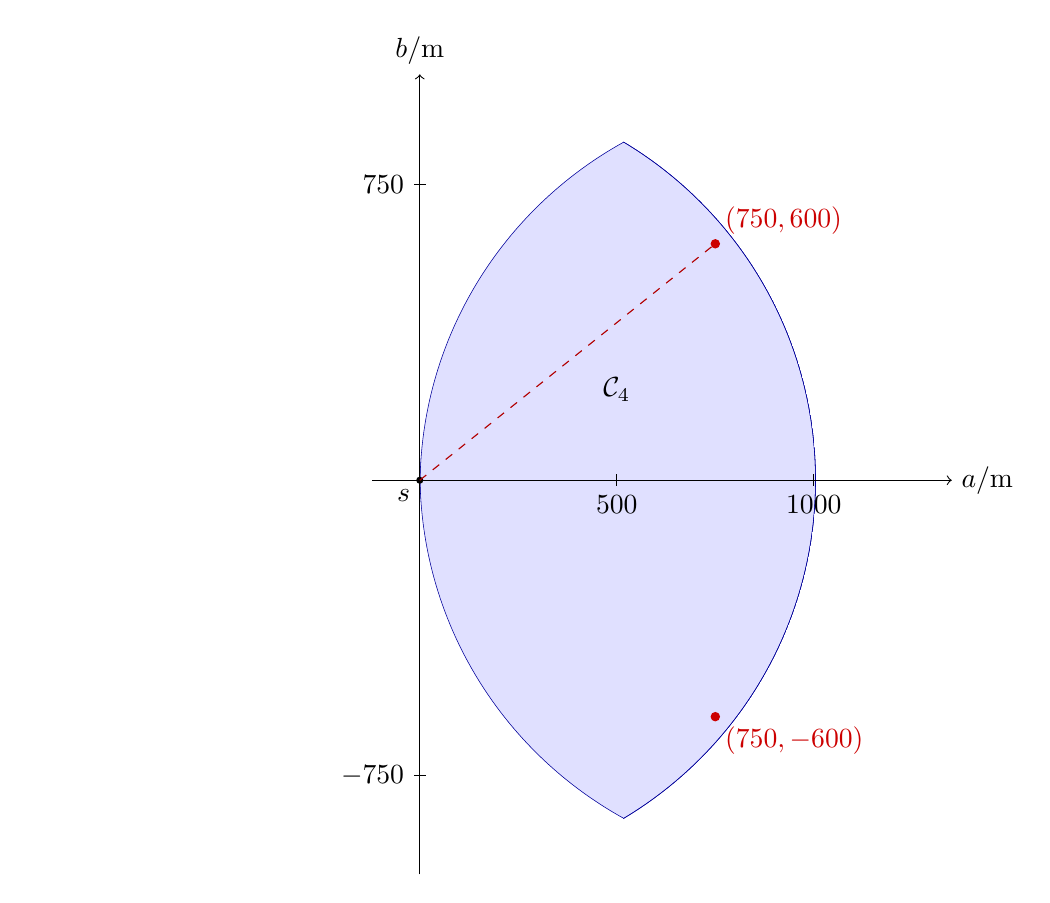
\begin{tikzpicture}[x=0.005cm,y=0.005cm]
  \begin{scope}
   \clip (4.99924,0.087262) circle[radius=1000];
   \clip (4.99924,-0.087262) circle[radius=1000];
   \clip (999.8477,17.4524) circle[radius=1000];
   \clip (999.8477,-17.4524) circle[radius=1000];
   \fill[blue!12] (-60,-1050) rectangle (1100,1050);
   \foreach \xx/\yy in {4.99924/0.087262,4.99924/-0.087262,999.8477/17.4524,999.8477/-17.4524}
    {\draw[blue!60!black] (\xx,\yy) circle[radius=1000];}
  \end{scope}
  \draw[->] (-120,0)--(1350,0) node[right] {$a/\mathrm{m}$};
  \draw[->] (0,-1000)--(0,1030) node[above] {$b/\mathrm{m}$};
  \foreach \x in {500,1000}{\draw (\x,15)--(\x,-15) node[below] {$\x$};}
  \foreach \y in {-750,750}{\draw (15,\y)--(-15,\y) node[left] {$\y$};}
  \fill (0,0) circle[radius=9] node[below left] {$s$};
  \draw[dashed,red!70!black] (0,0)--(750,600);
  \fill[red!80!black] (750,600) circle[radius=12] node[above right] {$(750,600)$};
  \fill[red!80!black] (750,-600) circle[radius=12] node[below right] {$(750,-600)$};
  \node at (500,230) {$\mathcal C_4$};
 \end{tikzpicture}
 \caption{首站局部坐标下的四圆保证接收区域，图取理论误差 $1^\circ$；标出一对可行示例点}
 \label{fig:b26-lens}
\end{figure}

\subsection{交会角对定位误差的影响}
设真实源到两站的距离为 $r_1,r_2$，两条视线单位向量为 $e_1,e_2$，夹角为 $\phi$。以 $n_1,n_2$ 表示对应单位法向量，小角误差下位置扰动满足近似关系
\begin{equation}
 N\Delta g=\eta,\qquad
 N=\begin{pmatrix}n_1^{\mathsf T}\\ n_2^{\mathsf T}\end{pmatrix},\qquad
 |\eta_i|\lesssim r_i\alpha,\qquad |\det N|=|\sin\phi|.
 \label{eq:b26-angle}
\end{equation}
当交会角接近 $0^\circ$ 或 $180^\circ$ 时，误差放大显著；较接近正交的交会通常更稳定。同时，离源越远，同样角误差对应的横向位置不确定性越大。因此，选点应同时关注交会角与第二站到可能目标的距离。

若目标恰在 $s+du$，取 $q=s+du+bv$ 可得到正交交会。但首观测并不知道 $d$，固定点不可能对整段可能距离都实现正交。本文据此在首方向两侧生成离轴候选，再用后验区域评价其表现，而不直接将某个固定三角形布局称为最优。

\subsection{有限候选与稳健评分}
首先在 $\mathcal C_4$ 内生成候选点，并施加设计移动预算 $\|q-s\|_2\leq L$，排除 $q=s$ 及横向基线过小的点。$L$ 是选点策略参数，不是题面限定。对一个假想目标 $g\in\mathcal G$ 及第二次角误差 $\varepsilon\in[-\alpha,\alpha]$，构造第二观测，并与首观测交会。

为了利用实际可用的先验，后验评价对象取
\begin{equation}
 K(q,g,\varepsilon)=W_1\cap W_2(q,g,\varepsilon)
 \cap\overline B(0,1800)\cap\overline B(s,1500)\cap\overline B(q,1500).
 \label{eq:b26-K}
\end{equation}
该集合可能具有圆弧边界，区别于问题一只含角约束的多边形 $P$。实现中使用圆的外接多边形，得到 $K\subseteq\widehat K$，再计算 $\widehat K$ 的最小包围圆半径。具体以 $64$ 边外接多边形表示目标圆域，以 $32$ 个切向半平面表示每个距离圆；所有近似均向外，避免把可能的真实目标错误排除。

连续稳健目标可定义为
\begin{equation}
 J(q)=\sup_{\substack{g\in\mathcal G\\|\varepsilon|\leq\alpha}}
 R^*\bigl(K(q,g,\varepsilon)\bigr).
\end{equation}
实际算法在有限场景集 $\mathcal S$ 上计算
\begin{equation}
 \widehat J(q)=\max_{(g,\varepsilon)\in\mathcal S}
 R^*\bigl(\widehat K(q,g,\varepsilon)\bigr).
 \label{eq:b26-score}
\end{equation}
若第二次反馈为近场，则该场景按半径 $5\,\mathrm{m}$ 的已知邻域计分，并直接清除。虽然每个已采样场景使用保守外近似，有限场景最大值仍不是连续 $J(q)$ 的已证明上界。

比较 $(\|q-s\|_2,\widehat J(q))$ 得到移动距离与定位精度的 Pareto 前沿。具体决策可采用：在 $\widehat J(q)\leq\tau$ 的候选中选最短移动点；若没有候选达到阈值，则选评分最小者。本文数值示例采用另一公开规则，即给定 $L=1000\,\mathrm{m}$，在该预算内先最小化 $\widehat J$，再以移动距离打破并列。全过程如下。
\begin{enumerate}
 \item 由首站和读数计算局部基、可能目标集合及四圆候选域。
 \item 生成有限离轴候选，按四圆约束、步长及横向阈值筛选。
 \item 对每个候选枚举假想目标和角误差场景，更新后验集合并计算其最小包围圆。
 \item 比较最坏采样半径与移动时间，按公开的预算或阈值选定下一站。
 \item 获得真实第二次反馈后重新更新区域；是否清除依据真实后验半径及接口结果决定。
\end{enumerate}
若候选数为 $M$、场景数为 $H$，主要评分开销为 $MH$ 次后验几何更新及最小圆计算。该计算属于现实程序开销，不计入式~\eqref{eq:b26-time}的虚拟移动和动作时间。

\subsection{候选点比较与数值结果}
取合成示例 $s=(0,0)$、$\theta=0^\circ$，使用实现误差界 $1.005^\circ$。候选网格为
\[
 a\in\{250,400,550,700,850\},\qquad
 b\in\{150,300,450,600,750\},
\]
筛去不满足接收约束者，加入解析可行点 $(750,600)$；另加入 $(500,0)$ 作为沿线退化对照，后者不参加正常离轴点选择。设横向阈值为 $100\,\mathrm{m}$，移动预算为 $1000\,\mathrm{m}$。评分使用 $18$ 个距离节点，包括 $5.001$、$1000$ 及 $1500$ 米附近边界，首角偏差和第二测向误差分别取 $\{-1^\circ,0^\circ,1^\circ\}$，每候选共 $162$ 个设计场景。

保持同一频道时，从首站到第二站的移动加检测时间为
\begin{equation}
 t_2(q)=\frac{\sqrt{a^2+b^2}}5+5.
 \label{eq:b26-cost2}
\end{equation}
表~\ref{tab:b26-q2}列出具有代表性的候选结果。均值是指定采样节点上的等权统计，不是题目环境的概率期望。
\begin{table}[htbp]
 \centering
 \caption{问题二合成示例中的部分候选点比较}\label{tab:b26-q2}
 \small
 \begin{tabular}{crrrr}
 \toprule
 $(a,b)/\mathrm{m}$ & 移动距离/米 & $t_2$/秒 & 最坏采样半径/米 & 平均采样半径/米 \\
 \midrule
 $(500,0)$（对照） & 500.00 & 105.00 & 500.19 & 341.41 \\
 $(250,150)$ & 291.55 & 63.31 & 251.28 & 95.07 \\
 $(400,300)$ & 500.00 & 105.00 & 136.68 & 46.64 \\
 $(550,450)$ & 710.63 & 147.13 & 87.89 & 31.99 \\
 $(550,600)$ & 813.94 & 167.79 & 74.10 & 29.51 \\
 $(700,600)$ & 921.95 & 189.39 & 63.04 & 27.18 \\
 $(750,600)$ & 960.47 & 197.09 & 59.63 & 26.75 \\
 $(850,450)$ & 961.77 & 197.35 & 60.55 & 27.75 \\
 \bottomrule
 \end{tabular}
\end{table}
在相同 $500\,\mathrm{m}$ 基线预算下，$(400,300)$ 的最坏采样半径显著小于沿线点 $(500,0)$，说明离轴交会能够有效压缩距离不确定性。按本例的预算优先规则，选中
\begin{equation}
 q^*=s+750u+600v,
\end{equation}
其最坏采样半径约 $59.631950\,\mathrm{m}$，移动加检测约 $197.093727\,\mathrm{s}$。该点优于本次枚举的其他合格候选，但不代表连续候选区域内的全局最优。

对选中点再采用 $63$ 个距离节点以及 $5\times5$ 组角偏差和误差组合复核，最坏采样半径仍为 $59.631950\,\mathrm{m}$。对全部候选进行 $301$ 个径向节点乘 $41$ 个角节点的接收检验，最大距离违反量为 $-26.484947\,\mathrm{m}$，均满足约束。对 $(550,450)$ 与其镜像点进行比较，最坏采样半径差约 $2.13\times10^{-13}\,\mathrm{m}$。接收可靠性由四圆解析证明保证，密集采样仅提供数值复核。

上述点的最坏采样半径仍大于 $20\,\mathrm{m}$，所以两次测向不能据此保证单点清除。第二问所得是一个可执行且保证接收的下一站策略，而非“两站必然精确定位”的结论。实际任务若更重视移动时间，可按时间预算或精度阈值选择较短基线点；其全任务收益应在后续搜索清除实验中比较。

\subsection{真实第二次反馈后的决策}
\begin{enumerate}
 \item 返回正常示向度：根据真实读数更新后验区域。若最小包围圆半径满足式~\eqref{eq:b26-clear}，前往其圆心清除；否则保留后验区域，交由后续测向或有限光学搜索继续处理。
 \item 返回近场：已知目标距当前站不超过 $5\,\mathrm{m}$，直接执行光学定位和清除，不再请求无意义的示向度。
 \item 返回无信号：在目标状态不变、全向且严格满足四圆条件的假设下，这与接收保证矛盾，应检查频道、源状态、数值边界及接口反馈。若主动选择四圆之外的探索点，则不能再宣称保证接收。
\end{enumerate}
如果首次观测与全局先验已经把目标约束在一个半径不超过 $20\,\mathrm{m}$ 的圆内，则无需机械执行第二次测向，可直接清除。一般首站可通过平移旋转构造四圆候选域，但全局目标圆心保持在原点，因此候选评分应按实际首站重算，不能将本例数值不加调整地移植到全部位置。

\clearpage
\endgroup
% ===== END B26 NEW MANUSCRIPT =====

% ===== ORIGINAL TEMPLATE BELOW: content preserved verbatim =====
\section*{原始模板与格式指导（原文保留）}
以下完整保留本项目原有模板内容，包括模板摘要、格式说明、示例图表、参考文献和附录代码，仅供后续排版与写作参考。此部分的示例问题、示例结论及声明文本均不属于前文 B 题模型与结果。

\noindent 前文新增内容包括问题重述、问题分析、模型假设与约定、符号说明，以及第一、二问的解答。后续第三、四问正文可继续添加在本分隔页之前。
\clearpage
\setcounter{section}{0}
\setcounter{subsection}{0}
\setcounter{equation}{0}
\setcounter{figure}{0}
\setcounter{table}{0}
\renewcommand{\thepage}{G-\arabic{page}}
\renewcommand{\theHsection}{guide.\arabic{section}}
\renewcommand{\theHequation}{guide.\arabic{equation}}
\renewcommand{\theHfigure}{guide.\arabic{figure}}
\renewcommand{\theHtable}{guide.\arabic{table}}
% ===== Original document body starts on the next line =====


 \maketitle
 \begin{abstract}
cumcmthesis 是为全国大学生数学建模竞赛编写的\LaTeX{}模板, 旨在让大家专注于 论文的内容写作, 而不用花费过多精力在格式的定制和调整上.  使用者需要有一 定的 \LaTeX{} 的使用经验, 至少要会使用常用宏包的一些功能, 比如参考文献，数学公式，图片使用，列表环境等等. 例子文件参看 \texttt{example.tex}.

\begin{framee}\small
  今年的格式变化如下：
\begin{itemize}
\item 更新了人工智能工具使用声明要求, 通知如下. 原文见 \url{https://www.mcm.edu.cn/html_cn/node/fef94648f2836ab6cc81586f4c38512b.html}
\end{itemize}
\setlength \fboxsep {1pt}
\fbox{\parbox{\linewidth-2.8pt}{\null
\begingroup
  \centering \bfseries
  全国大学生数学建模竞赛人工智能工具使用规定
  （2026年试行）\par
\endgroup\smallskip
\begin{enumerate}[label = \arabic*., topsep = 0pt, itemsep = 1pt]
  \item
  本规定适用于全国大学生数学建模竞赛中人工智能（以下简称 AI）工具
  的使用，包括但不限于大语言模型、生成式 AI、代码辅助工具和 AI智能
  体等。
  \item
  解决竞赛问题不要求必须使用 AI 工具。参赛队可在竞赛期间使用 AI 工
  具，但应遵循公开透明原则，确保参赛作品的核心建模与分析由参赛队
  主导，并对 AI 参与完成的内容逐项人工审查与核实。
  \item
  参赛队应在论文参考文献之前设置“AI 工具使用声明”
  ， 内容如下，二
  者择一：
  （1） 未使用 AI工具的，声明：“本参赛队在竞赛过程中未使用任何 AI
  工具。”
  （2） 使用 AI 工具的，声明：“本参赛队在竞赛过程中使用了 AI 工具，
  主要用于【简要用途，如语言润色、代码调试等】，详细使用情况
  见支撑材料。”
  \item
  使用AI工具的参赛作品，应在支撑材料中包含AI工具使用详情说明（PDF
  格式，文件名为“AI工具使用详情.pdf”），内容包括：
  （1） 所用AI 工具名称、版本或型号；
  （2） 具体使用目的和环节；
  （3） 主要提示方式与使用过程说明（可附典型交互示例）；
  （4） 对AI 输出的采纳、人工修改和核验的主要情况（语言润色除外）。
  \item
  不符合上述规定的参赛作品，视为违反竞赛规则，将根据情节轻重予以
  处理。故意隐瞒 AI使用情况、作出虚假声明，或者将未经必要人工审查
  与核实的AI 生成内容直接作为核心建模与分析成果提交的，取消其评奖
  资格。
  \item
  本规定自2026年9月 1日起试行。此前相关规定与本规定不一致的，以
  本规定为准。
  \item
  本规定由全国大学生数学建模竞赛组委会负责解释。
\end{enumerate}
}}

\end{framee}

\begin{center}
\begin{minipage}{.72\linewidth}
  \begin{itemize}
    \item
    网站\url{https://www.latexstudio.net} 陆续推出了更优质的资源，欢迎学习。
    \item
    欢迎大家到 QQ 群里沟通交流：91940767/200392395。问答区交流 \LaTeX{}技术：\url{https://ask.latexstudio.net}，有问题就来这里，与大神零距离。
    \item
    \uwave{右侧扫码关注我们的微信公众号}
  \end{itemize}
\end{minipage}
\hfill
\begin{minipage}{.24\linewidth}
  \centering
  
\includegraphics[width = \linewidth]{gongzhonghao2}
\end{minipage}
\end{center}

\keywords{\TeX{}\quad  图片\quad   表格\quad  公式}
\end{abstract}

%目录  2019 明确不要目录，我觉得这个规定太好了
%\tableofcontents

%\newpage

\section{模板的基本使用}

要使用 \LaTeX{} 来完成建模论文，首先要确保正确安装一个 \LaTeX{} 的发行版本。

\begin{itemize}
    \item Mac 下可以使用 Mac\TeX{}
    \item Linux 下可以使用 \TeX{}Live ；
    \item windows 下可以使用 \TeX{}Live 或者 Mik\TeX{} ;
\end{itemize}

具体安装可以参考 \href{https://github.com/OsbertWang/install-latex-guide-zh-cn/releases/}{Install-LaTeX-Guide-zh-cn} 或者其它靠谱的文章。另外可以安装一个易用的编辑器，例如 \href{https://mirrors.tuna.tsinghua.edu.cn/github-release/texstudio-org/texstudio/LatestRelease/}{\TeX{}studio} 。

使用该模板前，请阅读模板的使用说明文档。下面给出模板使用的大概样式。

\begin{tcode}
  \documentclass{cumcmthesis}
  % \documentclass[withoutpreface,bwprint]{cumcmthesis} %去掉封面与编号页

  \title{论文题目}
  \tihao{A}            % 题号
  \baominghao{4321}    % 报名号
  \schoolname{你的大学}
  \membera{成员A}
  \memberb{成员B}
  \memberc{成员C}
  \supervisor{指导老师}
  \yearinput{2017}     % 年
  \monthinput{08}      % 月
  \dayinput{22}        % 日

  \begin{document}
    \maketitle
    \begin{abstract}
      摘要的具体内容。
      \keywords{关键词1\quad  关键词2\quad   关键词3}
    \end{abstract}
    \tableofcontents
    \section{问题重述}
    \subsection{问题的提出}
    \section{模型的假设}
    \section{符号说明}
    \begin{center}
      \begin{tabular}{cc}
        \hline
        \makebox[.3\textwidth][c]{符号} &
        \makebox[.4\textwidth][c]{意义} \\ \hline
        D & 木条宽度（cm）\\ \hline
      \end{tabular}
    \end{center}
    \section{问题分析}
    \section{总结}
    \begin{thebibliography}{9}%宽度9
      \bibitem{bib:one} ....
    \end{thebibliography}
    \begin{appendices}
      附录的内容。
    \end{appendices}
  \end{document}
\end{tcode}

根据要求，电子版论文提交时需去掉封面和编号页。可以加上 \verb|withoutpreface|  选项来实现，即：
\begin{tcode}
    \documentclass[withoutpreface]{cumcmthesis}
\end{tcode}
这样就能实现了。打印的时候有超链接的地方不需要彩色，可以加上 \verb|bwprint| 选项。

另外目录也是不需要的，将 \verb|\tableofcontents| 注释或删除，目录就不会出现了。

团队的信息填入指定的位置，并且确保信息的正确性，以免因此白忙一场。

编译记得使用 \verb|xelatex|，而不是用 \verb|pdflatex|。在命令行编译的可以按如下方式编译：
\begin{tcode}
	xelatex example
\end{tcode}
或者使用 \verb|latexmk| 来编译，更推荐这种方式。
\begin{tcode}
	latexmk -xelatex example
\end{tcode}

下面给出写作与排版上的一些建议。

\section{图片}

建模中不可避免要插入图片。图片可以分为矢量图与位图。位图推荐使用 \verb|jpg,png| 这两种格式，避免使用 \verb|bmp| 这类图片，容易出现图片插入失败这样情况的发生。矢量图一般有 \verb|pdf,eps| ，推荐使用 \verb|pdf|  格式的图片，尽量不要使用 \verb|eps| 图片，理由相同。

注意图片的命名，避免使用中文来命名图片，可以用英文与数字的组合来命名图片。避免使用\verb|1,2,3| 这样顺序的图片命名方式。图片多了，自己都不清楚那张图是什么了，命名尽量让它有意义。下面是一个插图的示例代码。
\begin{figure}[!ht]
    \centering
    
\includegraphics[width=.6\textwidth]{smokeblk}
    \caption{电路图}
    \label{fig:circuit-diagram}
\end{figure}

注意 \verb|figure| 环境是一个浮动体环境，图片的最终位置可能会跑动。\verb|[!h]| 中的 \verb|h| 是 here 的意思， \verb|!| 表示忽略一些浮动体的严格规则。另外里面还可以加上 \verb|btp| 选项，它们分别是 bottom, top, page 的意思。只要这几个参数在花括号里面，作用是不分先后顺序的。page 在这里表示浮动页。

\verb|\label{fig:circuit-diagram}| 是一个标签，供交叉引用使用的。例如引用图片 \verb|\cref{fig:circuit-diagram}| 的实际效果是\cref{fig:circuit-diagram}。图片是自动编号的，比起手动编号，它更加高效。\verb|\cref{label}| 由 \verb|cleveref| 宏包提供，比普通的 \verb|\ref{label}| 更加自动化。 \verb|label| 要确保唯一，命名方式推荐用图片的命名方式。

图片并排的需求解决方式多种多样，下面用 \verb|minipage| 环境来展示一个简单的例子。注意，以下例子用到了 \verb|subcaption| 命令，需要加载 subcaption 宏包。

\begin{figure}
    \centering
    \begin{minipage}[c]{0.3\textwidth}
        \centering
        
\includegraphics[width=0.95\textwidth]{f1}
        \subcaption{流程图}
        \label{fig:sample-figure-a}
    \end{minipage}
    \begin{minipage}[c]{0.3\textwidth}
        \centering
        
\includegraphics[width=0.95\textwidth]{f1}
        \subcaption{流程图}
        \label{fig:sample-figure-b}
    \end{minipage}
    \begin{minipage}[c]{0.3\textwidth}
        \centering
        
\includegraphics[width=0.95\textwidth]{f1}
        \subcaption{流程图}
        \label{fig:sample-figure-c}
    \end{minipage}
    \caption{多图并排示例}
    \label{fig:sample-figure}
\end{figure}
这相当于整体是一张大图片，大图片引用是\cref{fig:sample-figure}，子图引用别分是\cref{fig:sample-figure-a}、\cref{fig:sample-figure-b}、\cref{fig:sample-figure-c}。

如果原本两张图片的高度不同，但是希望它们缩放后等高的排在同一行，参考这个例子：
\begin{figure}
    \centering
    \begin{minipage}[c]{0.48\textwidth}
        \centering
        
\includegraphics[height=0.2\textheight]{cat}
        \subcaption{一只猫}
    \end{minipage}
    \begin{minipage}[c]{0.48\textwidth}
        \centering
        
\includegraphics[height=0.2\textheight]{smokeblk}
        \subcaption{电路图}
    \end{minipage}
    \caption{多图并排示例}
\end{figure}

\section{绘制普通三线表格}
表格应具有三线表格式，因此常用 booktabs宏包，其标准格式如\cref{tab:001}~所示。
\begin{table}[!htbp]
    \caption{标准三线表格}\label{tab:001} \centering
    \begin{tabular}{ccccc}
        \toprule[1.5pt]
        $D$(in) & $P_u$(lbs) & $u_u$(in) & $\beta$ & $G_f$(psi.in)\\
        \midrule[1pt]
        5 & 269.8 & 0.000674 & 1.79 & 0.04089\\
        10 & 421.0 & 0.001035 & 3.59 & 0.04089\\
        20 & 640.2 & 0.001565 & 7.18 & 0.04089\\
        \bottomrule[1.5pt]
    \end{tabular}
\end{table}

其绘制表格的代码及其说明如下。
\begin{tcode}
    \begin{table}[!htbp]
        \caption[标签名]{中文标题}
        \begin{tabular}{cc...c}
            \toprule[1.5pt]
            表头第1个格   & 表头第2个格   & ... & 表头第n个格  \\
            \midrule[1pt]
            表中数据(1,1) & 表中数据(1,2) & ... & 表中数据(1,n)\\
            表中数据(2,1) & 表中数据(2,2) & ... & 表中数据(2,n)\\
            ...................................................\\
            表中数据(m,1) & 表中数据(m,2) & ... & 表中数据(m,n)\\
            \bottomrule[1.5pt]
        \end{tabular}
    \end{table}
\end{tcode}

\bigskip

table环境是一个将表格嵌入文本的浮动环境。tabular环境的必选参数由每列对应一个格式字符所组成：c表示居中，l表示左对齐，r表示右对齐，其总个数应与表的列数相同。此外，\verb|@{文本}|可以出现在任意两个上述的列格式之间，其中的文本将被插入每一行的同一位置。表格的各行以\verb|\\|分隔，同一行的各列则以\&分隔。 \verb|\toprule| 、\verb|\midrule| 和 \verb|\bottomrule| 三个命令是由booktabs宏包提供的，其中 \verb|\toprule| 和 \verb|\bottomrule| 分别用来绘制表格的第一条（表格最顶部）和第三条（表格最底部）水平线， \verb|\midrule| 用来绘制第二条（表头之下）水平线，且第一条和第三条水平线的线宽为 1.5pt ，第二条水平线的线宽为 1pt 。引用方法与图片的相同。

\section{公式}

数学建模必然涉及不少数学公式的使用。下面简单介绍一个可能用得上的数学环境。

首先是行内公式，例如 $ \theta $ 是角度。行内公式使用 \verb|$  $| 包裹。

行间公式不需要编号的可以使用 \verb|\[  \]| 包裹，例如
\[
E=mc^2
\]
其中 $ E $ 是能量，$ m $ 是质量，$ c $ 是光速。

如果希望某个公式带编号，并且在后文中引用可以参考下面的写法：
\begin{equation}
E=mc^2
\label{eq:energy}
\end{equation}
式\cref{eq:energy}是质能方程。

多行公式有时候希望能够在特定的位置对齐，以下是其中一种处理方法。
\begin{align}
P & = UI \\
& = I^2R
\end{align}
\verb|&| 是对齐的位置， \verb|&| 可以有多个，但是每行的个数要相同。

矩阵的输入也不难。
\[
\mathbf{X} = \left(
    \begin{array}{cccc}
    x_{11} & x_{12} & \ldots & x_{1n}\\
    x_{21} & x_{22} & \ldots & x_{2n}\\
    \vdots & \vdots & \ddots & \vdots\\
    x_{n1} & x_{n2} & \ldots & x_{nn}\\
    \end{array} \right)
\]

分段函数这些可以用 \verb|case| 环境，但是它要放在数学环境里面。
\[
f(x) =
    \begin{cases}
        0 &  x \text{为无理数} ,\\
        1 &  x \text{为有理数} .
    \end{cases}
\]
在数学环境里面，字体用的是数学字体，一般与正文字体不同。假如要公式里面有个别文字，则需要把这部分放在 \verb|text| 环境里面，即 \verb|\text{文本环境}| 。

公式中个别需要加粗的字母可以用 \verb|$\bm{math symbol}$| 。如 $ \alpha a\bm{\alpha a} $ 。

以上仅简单介绍了基础的使用，对于更复杂的需求，可以阅读相关的宏包手册，如 \href{http://texdoc.net/texmf-dist/doc/latex/amsmath/amsldoc.pdf}{amsmath}。

希腊字母这些如果不熟悉，可以去查找符号文件 \href{http://mirrors.ctan.org/info/symbols/comprehensive/symbols-a4.pdf}{symbols-a4.pdf} ，也可以去 \href{http://detexify.kirelabs.org/classify.html}{detexify} 网站手写识别。另外还有数学公式识别软件 \href{https://mathpix.com/}{mathpix} 。

下面简单介绍一下定理、证明等环境的使用。
\begin{definition}
    定义环境
    \label{def:nosense}
\end{definition}
\cref{def:nosense}除了告诉你怎么使用这个环境以外，没有什么其它的意义。

除了 definition 环境，还可以使用 theorem 、lemma、corollary、assumption、conjecture、axiom、principle、problem、example、proof、solution 这些环境，根据论文的实际需求合理使用。

\begin{theorem}
    这是一个定理。
    \label{thm:example}
\end{theorem}
由\cref{thm:example}我们知道了定理环境的使用。

\begin{lemma}
    这是一个引理。
    \label{lem:example}
\end{lemma}
由\cref{lem:example}我们知道了引理环境的使用。

\begin{corollary}
    这是一个推论。
    \label{cor:example}
\end{corollary}
由\cref{cor:example}我们知道了推论环境的使用。

\begin{assumption}
    这是一个假设。
    \label{asu:example}
\end{assumption}
由\cref{asu:example}我们知道了假设环境的使用。

\begin{conjecture}
    这是一个猜想。
    \label{con:example}
\end{conjecture}
由\cref{con:example}我们知道了猜想环境的使用。

\begin{axiom}
    这是一个公理。
    \label{axi:example}
\end{axiom}
由\cref{axi:example}我们知道了公理环境的使用。

\begin{principle}
    这是一个定律。
    \label{pri:example}
\end{principle}
由\cref{pri:example}我们知道了定律环境的使用。

\begin{problem}
    这是一个问题。
    \label{pro:example}
\end{problem}
由\cref{pro:example}我们知道了问题环境的使用。

\begin{example}
    这是一个例子。
    \label{exa:example}
\end{example}
由\cref{exa:example}我们知道了例子环境的使用。

\begin{proof}
    这是一个证明。
    \label{prf:example}
\end{proof}
由\cref{prf:example}我们知道了证明环境的使用。

\begin{solution}
    这是一个解。
    \label{sol:example}
\end{solution}
由\cref{sol:example}我们知道了解环境的使用。



\section{其它小功能}
\subsection{脚注}

利用 \verb|\footnote{具体内容}| 可以生成脚注\footnote{脚注可以补充说明一些东西}。

\subsection{无序列表与有序列表}

无序列表是这样的：
\begin{itemize}
    \item one
    \item two
    \item ...
\end{itemize}

有序列表是这样子的：
\begin{enumerate}
    \item one
    \item two
    \item ...
\end{enumerate}

\subsection{字体加粗与斜体}

如果想强调部分内容，可以使用加粗的手段来实现。加粗字体可以用 \verb|\textbf{加粗}| 来实现。例如： \textbf{这是加粗的字体。 This is bold fonts} 。

中文字体没有斜体设计，但是英文字体有。\textit{斜体 Italics}。

\section{参考文献与引用}

参考文献对于一篇正式的论文来说是必不可少的，在建模中重要的参考文献当然应该列出。\LaTeX{}在这方面的功能也是十分强大的，下面进介绍一个比较简单的参考文献制作方法。有兴趣的可以学习 \verb|bibtex| 或 \verb|biblatex| 的使用。

\LaTeX{}的入门书籍可以看《\LaTeX{}入门》\cite{liuhaiyang2013latex}。这是一个简单的引用，用 \verb|\cite{bibkey}| 来完成。要引用成功，当然要维护好 bibitem 了。下面是个简单的例子。


若未使用 AI, 需要在参考文献前使用命令~\verb|\CumcmAINotUsed| 加入如下段落:

\CumcmAINotUsed

若使用了 AI, 需要使用命令 \verb|\CumcmAIUsed{<用途>}| 加入如下段落:
\CumcmAIUsed{[简要用途, 如语言润色, 代码调试等]}

支撑材料格式如下.

\section*{AI工具使用详情}

\subsection*{工具信息}
\noindent
\begin{tabularx}{\textwidth}{@{}XX@{}}
  \toprule
  项目 & 填写内容 \\
  \midrule
  工具名称 & \textit{填写实际使用的产品或工具名称} \\
  版本或型号 & \textit{填写实际版本、模型名称或可识别的型号} \\
  使用日期 & \textit{YYYY-MM-DD 至 YYYY-MM-DD} \\
  \bottomrule
\end{tabularx}

\subsection*{具体使用目的和环节}
逐项说明 AI 用于语言润色、代码调试、资料整理或其他环节；不得笼统写“辅助论文”。明确其输入、输出及对应论文位置。

\subsection*{主要提示方式与使用过程}
说明主要提示策略与迭代过程，可附具有代表性的交互片段。不要包含参赛者姓名、学校或赛区信息。

\subsection*{采纳、人工修改与核验}
除语言润色外，逐项记录 AI 输出是否采纳、由谁进行何种人工修改、采用何种数据或实验复核，以及最终结论是否发生变化。

\subsection*{人工核验清单}
\begin{enumerate}[label=\arabic*)]
  \item 核对公式推导、单位、边界条件和符号一致性；
  \item 在独立环境中运行全部代码并复现论文表图；
  \item 核验引用、数据来源和事实陈述；
  \item 确认核心建模与分析由参赛队主导；
  \item 确认论文声明与本详情文件一致。
\end{enumerate}


%参考文献
\begin{thebibliography}{9}%宽度9
    \bibitem[1]{liuhaiyang2013latex}
    刘海洋.
    \newblock \LaTeX {}入门\allowbreak[J].
    \newblock 电子工业出版社, 北京, 2013.
    \bibitem[2]{mathematical-modeling}
    全国大学生数学建模竞赛论文格式规范 (2023 年 修改).
    \bibitem{3} \url{https://www.latexstudio.net}
\end{thebibliography}
  
\newpage
%附录
\begin{appendices}

\section{模板所用的宏包}
\begin{table}[htbp]
    \centering
    \caption{宏包罗列}
    \begin{tabular}{ccccc}
        \toprule
        \multicolumn{5}{c}{模板中已经加载的宏包} \\
        \midrule
        amsbsy & amsfonts & {amsgen} & {amsmath} & {amsopn} \\
        amssymb & amstext & {appendix} & {array} & {atbegshi} \\
        atveryend & auxhook & {bigdelim} & {bigintcalc} & {bigstrut} \\
        bitset & bm    & {booktabs} & {calc} & {caption} \\
        caption3 & CJKfntef & {cprotect} & {ctex} & {ctexhook} \\
        ctexpatch & enumitem & {etexcmds} & {etoolbox} & {everysel} \\
        expl3 & fix-cm & {fontenc} & {fontspec} & {fontspec-xetex} \\
        geometry & gettitlestring & {graphics} & {graphicx} & {hobsub} \\
        hobsub-generic & hobsub-hyperref & {hopatch} & {hxetex} & {hycolor} \\
        hyperref & ifluatex & {ifpdf} & {ifthen} & {ifvtex} \\
        ifxetex & indentfirst & {infwarerr} & {intcalc} & {keyval} \\
        kvdefinekeys & kvoptions & {kvsetkeys} & {l3keys2e} & {letltxmacro} \\
        listings & longtable & {lstmisc} & {ltcaption} & {ltxcmds} \\
        multirow & nameref & {pdfescape} & {pdftexcmds} & {refcount} \\
        rerunfilecheck & stringenc & {suffix} & {titletoc} & {tocloft} \\
        trig  & ulem  & {uniquecounter} & {url} & {xcolor} \\
        xcolor-patch & xeCJK & {xeCJKfntef} & {xeCJK-listings} & {xparse} \\
        xtemplate & zhnumber &       &       &  \\
        \bottomrule
    \end{tabular}%
    \label{tab:addlabel}%
\end{table}%

以上宏包都已经加载过了，不要重复加载它们。

\section{排队算法--matlab 源程序}

\begin{lstlisting}[language=matlab]
kk=2;[mdd,ndd]=size(dd);
while ~isempty(V)
[tmpd,j]=min(W(i,V));tmpj=V(j);
for k=2:ndd
[tmp1,jj]=min(dd(1,k)+W(dd(2,k),V));
tmp2=V(jj);tt(k-1,:)=[tmp1,tmp2,jj];
end
tmp=[tmpd,tmpj,j;tt];[tmp3,tmp4]=min(tmp(:,1));
if tmp3==tmpd, ss(1:2,kk)=[i;tmp(tmp4,2)];
else,tmp5=find(ss(:,tmp4)~=0);tmp6=length(tmp5);
if dd(2,tmp4)==ss(tmp6,tmp4)
ss(1:tmp6+1,kk)=[ss(tmp5,tmp4);tmp(tmp4,2)];
else, ss(1:3,kk)=[i;dd(2,tmp4);tmp(tmp4,2)];
end;end
dd=[dd,[tmp3;tmp(tmp4,2)]];V(tmp(tmp4,3))=[];
[mdd,ndd]=size(dd);kk=kk+1;
end; S=ss; D=dd(1,:);
 \end{lstlisting}

未使用 AI 使用cheng bi sai zh使用了 AI wei shi yong

 \section{规划解决程序--lingo源代码}

\begin{lstlisting}[language=c]
kk=2;
[mdd,ndd]=size(dd);
while ~isempty(V)
    [tmpd,j]=min(W(i,V));tmpj=V(j);
for k=2:ndd
    [tmp1,jj]=min(dd(1,k)+W(dd(2,k),V));
    tmp2=V(jj);tt(k-1,:)=[tmp1,tmp2,jj];
end
    tmp=[tmpd,tmpj,j;tt];[tmp3,tmp4]=min(tmp(:,1));
if tmp3==tmpd, ss(1:2,kk)=[i;tmp(tmp4,2)];
else,tmp5=find(ss(:,tmp4)~=0);tmp6=length(tmp5);
if dd(2,tmp4)==ss(tmp6,tmp4)
    ss(1:tmp6+1,kk)=[ss(tmp5,tmp4);tmp(tmp4,2)];
else, ss(1:3,kk)=[i;dd(2,tmp4);tmp(tmp4,2)];
end;
end
    dd=[dd,[tmp3;tmp(tmp4,2)]];V(tmp(tmp4,3))=[];
    [mdd,ndd]=size(dd);
    kk=kk+1;
end;
S=ss;
D=dd(1,:);
 \end{lstlisting}
\end{appendices}

\end{document} 